\chapter{Event Reconstruction}\label{chap:pflow}

\section{Introduction}
\label{sec:ch4:intro}




Particle flow CITE is the name given to the algorithms that take information from each of the subdetectors to reconstruct complete trajectories of most particles produced in collisions. The objects that can be identified by particle flow are the photon, charged and neutral hadrons (reconstructed as jets), the muon, and the electron. Neutrinos are not detected by CMS. Particle flow is used in CMS but was developed years before for the LEP experiment at CERN CITE.

In the ECAL charged and neutral hadrons cannot be distinguished from one another. Charged and neutral hadrons leave about 25\% of their energy in the ECAL.


Particle flow combines tracks form the tracker, vertices, and energy deposits in the ECAL and HCAL, and tracks from the muon system. The hits in the ECAL and HCAL are clustered to estimate the energy and direction of the particles. Photons are reconstructed mostly from information in the ECAL, and electrons from the tracker and ECAL. 

The resolutions of the subdetectors do mot have the same coarseness. The tracker has a much finer resolution, while the ECAL and HCAL have a coarser resolution.

 \begin{figure}[h]
\centering
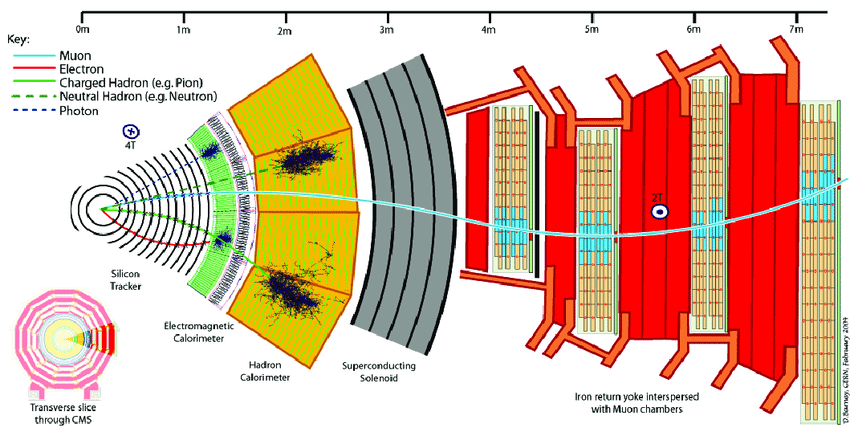
\includegraphics[width=0.9\textwidth]{figures/cms_slice}
\caption{A slice of CMS depicting the trajectory of a charged particle and its deposits in the subdetectors.}
\label{fig:cms_slice}
\end{figure}

\section{Reconstructing Charged Particles}


Charged particles are detected in the first layer of CMS, the silicone tracker. The particle tracks are reconstructed using a combinatorial track finder, which uses a randomly generated track to find the hits compatible with the detected charged-particle trajectory. 


The particle flow algorithm reconstructs tracks using iterative tracking. First, a combinatorial track finder constructs a track in 3 steps:

\begin{enumerate}
	\item Initial seed generation using hits from the tracker
	\item Collecting hits that fall within the constructed track from Step 1
	\item Final fit of the track to calculate the $p_T$ and origin of the object
\end{enumerate}


To reduce misreconstruction of tracks, this combinatorial track finding is done several times with more critera applied each time. The hits that have already been assigned to tracks are also removed from consideration in future iterations. Additional criteria are placed on 

\begin{itemize}
	\item $\chi^2$ of the fit
	\item track compatibility with reconstructed primary vertex
	\item track seeds
	\item track kinematics
	\item number of hits
\end{itemize}

In the first iteration, if a track with 8 hits and no more than one missing hit is found it is considered a reconstructed track and no further criteria is used. The track reconstruction algorithm goes through 10 iterations, first starting with tracks with 3 pixel hits, then on tracks with less pixel hits, then tracks with only hits in the strips, then looking for muons using information from the muon detector system.

\section{Reconstructing Electrons}

Electrons leave a track in tracker, and then when it reaches the ECAL, it deposits its energy as well as the energy of the radiating bremsstrahlung photons, which results in a supercluster in the ECAL which must be detected as coming from one electron. However this is difficult to do in practice, as energy deposits from other particles in the ECAL often overlap with the electron’s supercluster.


\section{Reconstructing Photons}

Photons appear in the detector similarly to electrons but without a track. In the ECAL, the requirements for electrons and photons are the same. A photon must be isolated from the calorimeter deposits of charged particles in the ECAL and HCAL.

\section{Reconstructing Muons}

The CMS detector is built to reconstruct muons as accurately as possible. The muon reconstruction is very efficient, with 99\% of muons accurately reconstructed. There can be false positives in the PF reconstruction of a muon, since some hadrons can punch through and be detected in the muon system. With multiple subdetectors able to identify muons, there are three ways muons are reconstructed that allows for PF reconstruction of the muon. Muons that are reconstructed in the tracker alone are called “tracker muons”. Muons that are reconstructed only in the muon detectors - the drift tubes or the cathode strip chambers - are called “standalone muons”. Muons that are reconstructed using all subdetectors are “global muons". Global muon reconstruction is the most efficient of the muon reconstructions when the muon $p_T$ is greater than 10 GeV.

In order to distinguish between muons from $q\bar{q}$ decays and muons from W and Z decays, tighter muon identification requirements are given to identify the latter events. A "soft muon" is a tracker muon with 1 pixel hit and at least 4 other inner tracker hits. The "tight muon" is a soft muon with a $\chi^2/dof < 10$, at least one hit in the muon system, and 2 matched muon segments in the muon station, the section of the muon system surrounding the solenoid. CITE


\section{Jets}

Figure~\ref{fig:pflow_jets} shows a sketch of how the energy deposits in the ECAL and HCAL appear for the object they are associated with. Muons leave effectively no energy deposits in the calorimeters, neutral hadrons and photons leave no tracks but leave energy deposits in the HCAL and ECAL, respectively. And charged hadrons and electrons have tracks associated with their energy deposits in the calorimeters.


\begin{figure}[h]
\centering
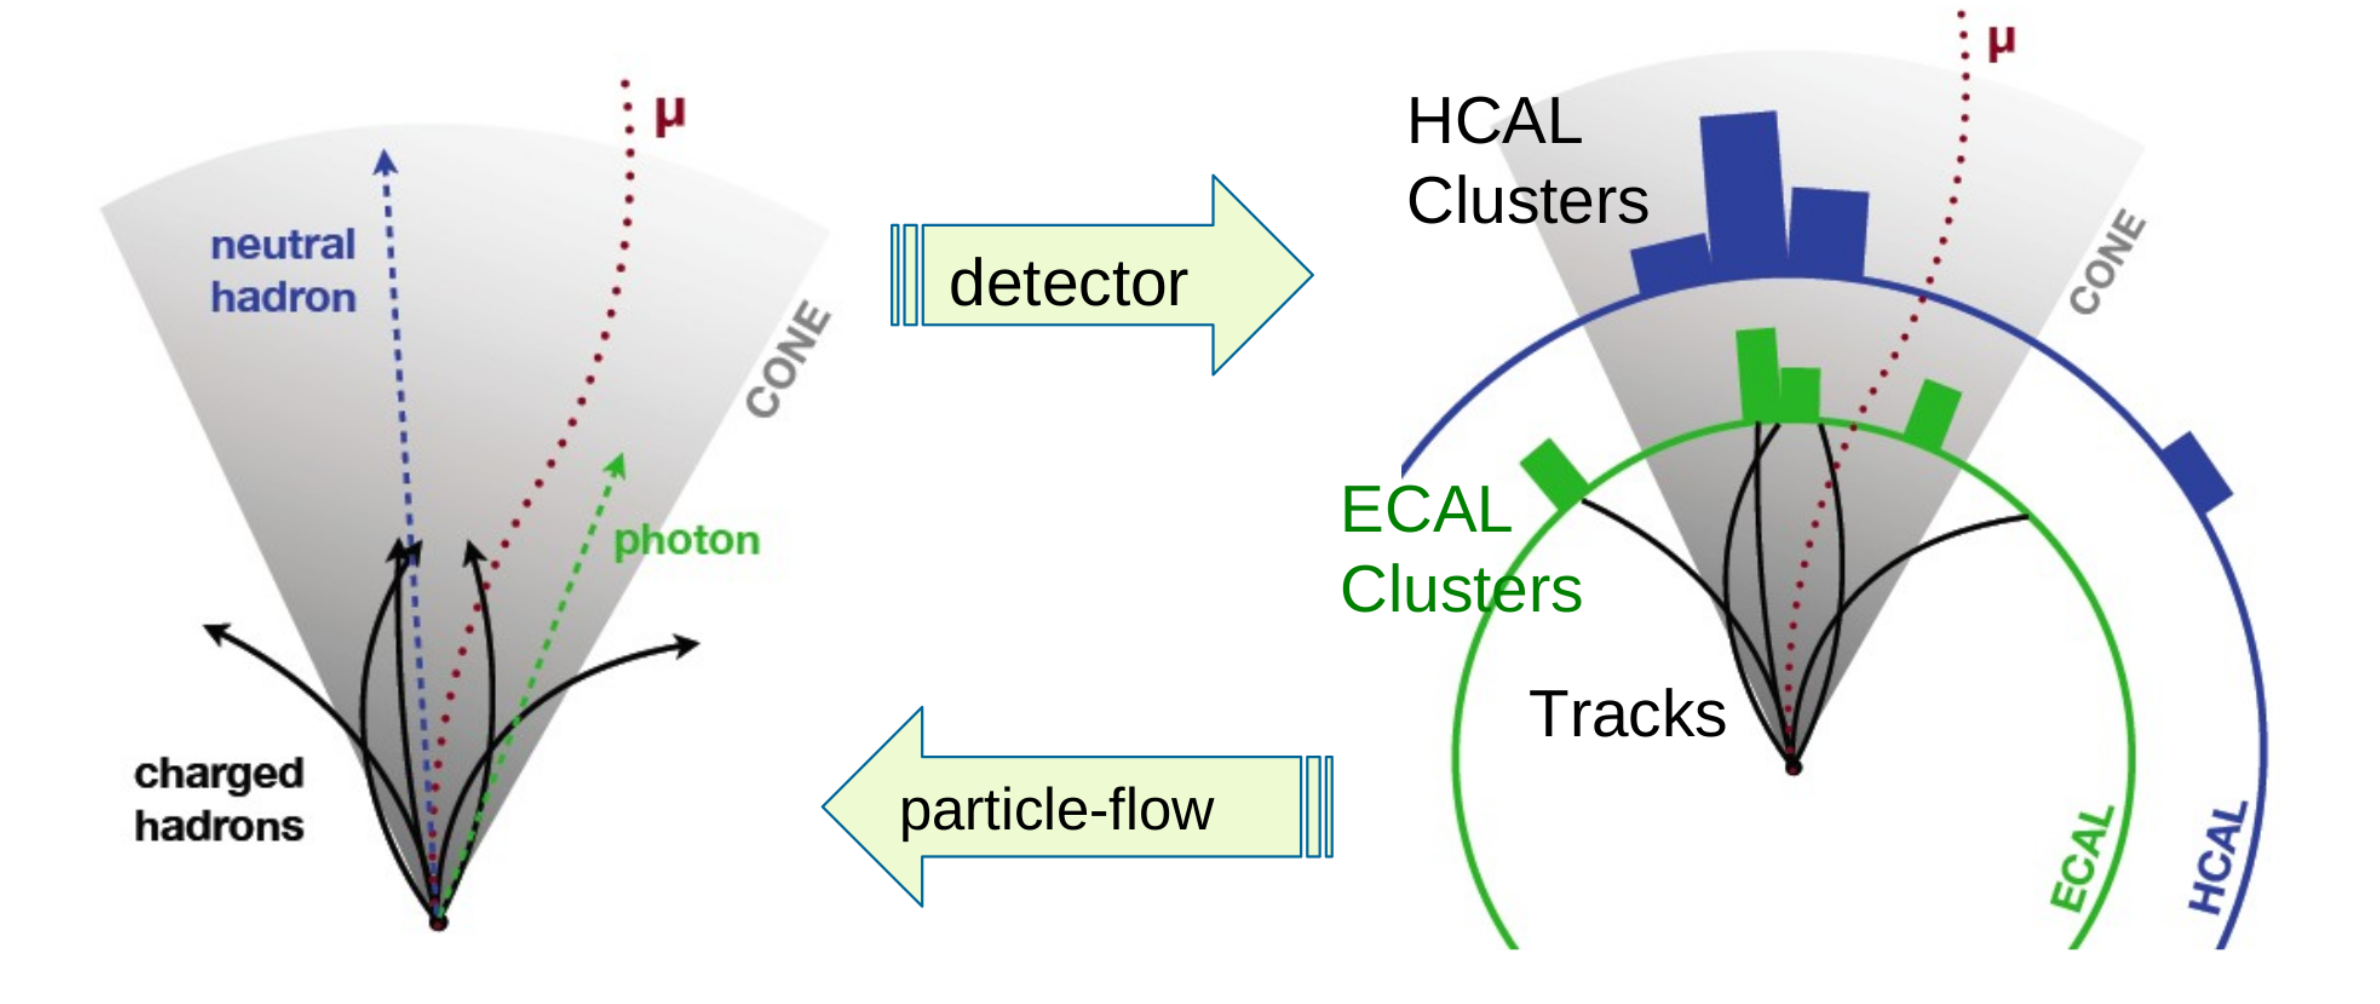
\includegraphics[width=1.0\textwidth]{figures/particle_flow_pandolfi}
\caption{A diagram of particle flow reconstruction of jets in the CMS detector~\cite{pflow_pandolfi}.}
\label{fig:pflow_jets}
\end{figure}

Jets are reconstructed using a clustering algorithm. The jet clustering algorithm used in this analysis is the anti-kt algorithm. The jets clustered by the anti-kt algorithm and with a radius parameter of R=0.4 are called AK4 jets.

The anti-kt algorithm works favors clustering a particle with the nearest hard particle~\cite{anti-kt}. This ensures that soft particles are less likely to be clustered together. The algorithm for anti-kt clustering comes from the same equation used for Cambridge/Aachen clustering:

\begin{equation}
	d_{ij} = \text{min} \left( k^{2p}_{ti}, k^{2p}_{tj} \right) \frac{\Delta^2_{ij}}{R^2}
\end{equation}
\begin{equation}
	d_{iB} = k^{2p}_{ti}
\end{equation}
\begin{equation}
	\Delta_{ij} = (y_i - y_j)^2 + (\phi_i - \phi_j)^2
\end{equation}

where $k_{ti}$ ($k_{tj}$) is transverse momentum, $y_i$ ($y_j$) is rapidity, and $\phi_i$ ($\phi_j$) is the azimuthal angle of the ith (jth) particle.

The AK4 jets can be reconstructed from only the ECAL and HCAL clusters. These jets are referred to as Calo Jets. The AK4 jets reconstructed with all of the particle flow information are called PF Jets. The jets reconstructed using all of the particles produced by an MC event generator are called Gen Jets. 


A diagram of these PF, Calo, and Gen jets is shown in Figure~\ref{fig:pfjet} and a graphic of particle flow reconstruction is shown in Figure~\ref{fig:pflow_jets}.


PF Jets are jets reconstructed using all particle flow candidates. PF+CHS Jets are reconstructed using all particle flow candidates except the charged hadrons associated with a pileup primary vertex. Gen Jets are jets generated from Monte Carlo simulation. Calo jets are jets made by clustering the sum of energy deposits in the ECAL and HCAL detectors.. A PF, Calo, and Ref jet for the same event are shown in the diagram for Figure~\ref{fig:pfjet}.

\begin{figure}[h]
\centering
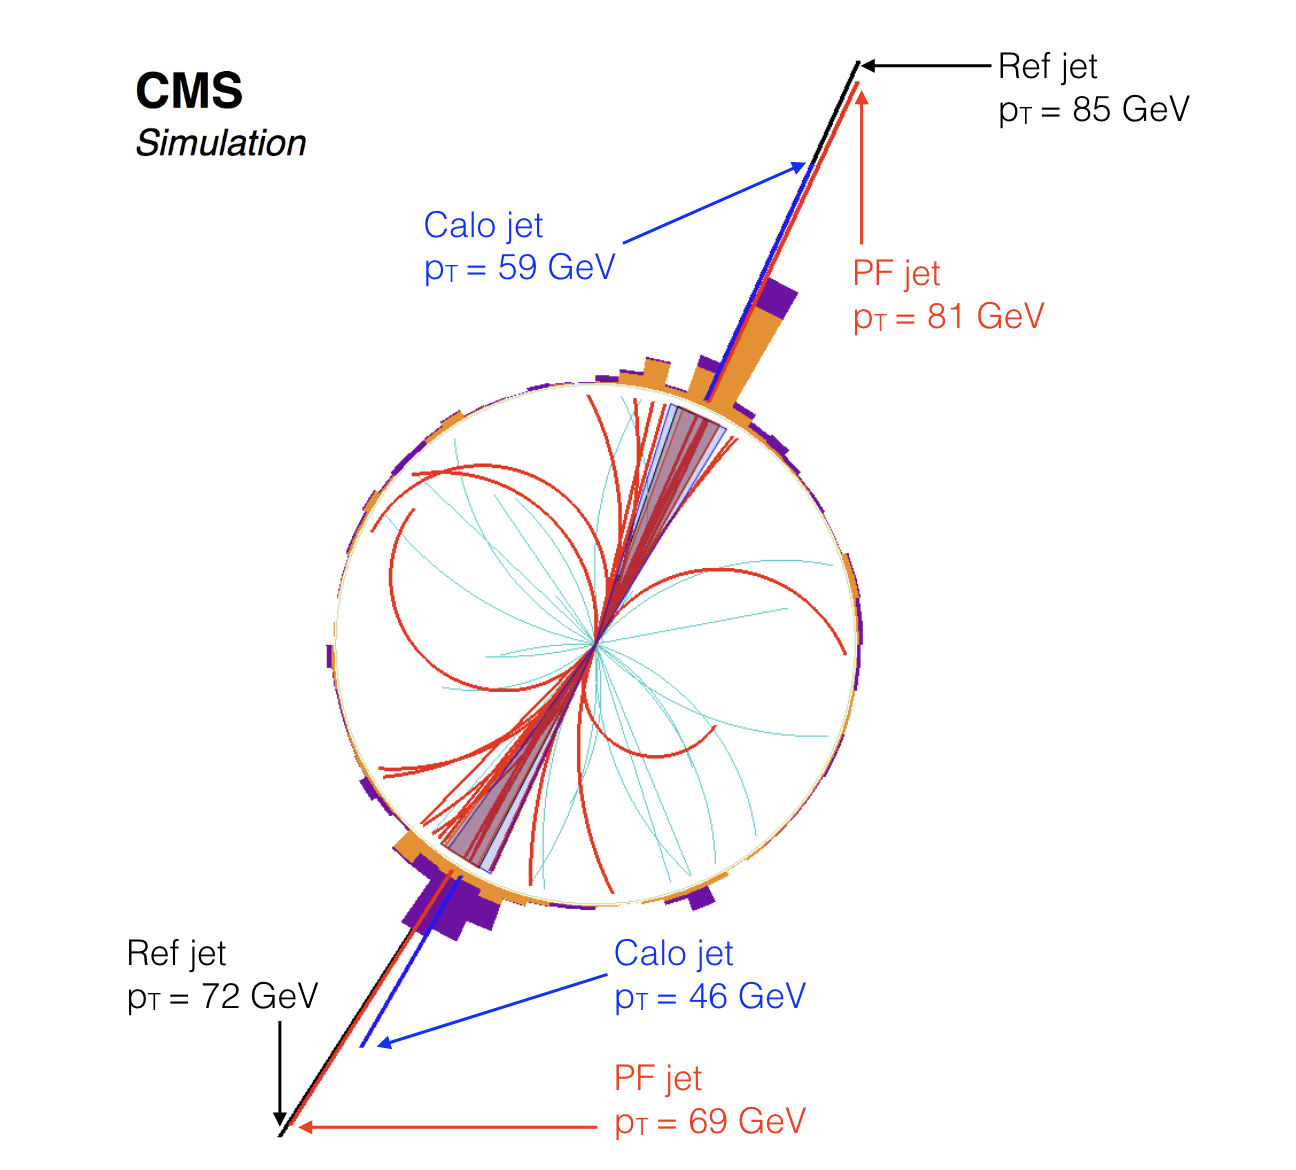
\includegraphics[width=0.9\textwidth]{figures/pf_jet_diagram}
\caption{A diagram of a dijet event and the reconstruction of the PF, Calo, and Gen (labelled as "Ref") jets~\cite{pflow}.}
\label{fig:pfjet}
\end{figure}


\subsection{Softdrop jet mass}

One of the observables in this analysis is the soft drop mass of the AK8 jets. The soft drop algorithm recursively removes soft particles which helps to distinguish boosted jets from background QCD jets. Both jets in the event are therefore required to pass the soft drop conditions~\cite{softdrop}:
	
%with a separation of $\Delta \phi > 2.1$. The semileptonic analysis requires exactly 1 top-tagged AK8 jet and hence is forced to be orthognal. Our event selection does not have dilepton events and are therefore also orthogonal to the dileptonic analysis of this channel. 

%The signal region is defined by the two jets in the ttbar candidate passing the top tagger, and by a soft drop mass window cut of $105 < m_{SD} < 210 GeV$. The sidebands of the soft drop mass are $25 < m_{SD} < 105 GeV$ and $210 < m_{SD} < 475 GeV$ and are used for background estimation. Both jets in the event are therefore required to pass the soft drop conditions:

\begin{itemize}

	\item Undo the last stage of Cambridge-Aachen clustering to to break the jet $j$ into two subjets $j_1$ and $j_2$.
	\item Require both subjets to pass the soft drop condition
	
	\begin{equation}
		   \frac {\text{min}(p_{T1},p_{T2} )}{p_{T1} + p_{T2}} >   z_{\text{cut}} \left( \frac{ \Delta R_{12} }{ R_0 } \right)^{\beta}
	\end{equation}
	
	where $p_{T1}$ and $p_{T2}$ are the $p_{T}$ of $j_1$ and $j_2$, respectively; $\Delta R_{12}$ is the distance between $j_1$ and $j_2$ in the rapidity-azimuth plane, $R_0$ is the jet radius, and $z_{\text{cut}}$ = 0.1 is the soft drop threshold, and $\beta$ = 0 is the angular exponent. 
	
	\item If the subjets pass the soft drop condition, define $j$ as the final state soft drop jet. If the subjets fail the condition, redefine the subjet with the larger $p_T$ as $j$ and iterate the soft drop algorithm.
	
\end{itemize}



\section{Missing $p_T$}

The missing $p_T$ is useful for the identification of neutrinos which do not interact with any of the detector materials. It can also be useful to search for new particles. The sum of the $p_T$ in the azimuthal plane is 0 before an event, which means event in which $\sum p_{T} > 0$ has missing $p_T$. Missing $p_T$ is defined in Equation~\ref{eq:ptmiss} before jet energy corrections, and in Equation~\ref{eq:ptmiss_corr} after corrections.

\begin{equation}
	p^{miss}_{T}   = -\sum_{i=1}^{N_{particles}} p_{T_{i}}
	\label{eq:ptmiss}
\end{equation}

\begin{equation}
	p^{miss}_{T,PF}   = -\sum_{i=1}^{N_{particles}} p_{T_{i}} - \sum_{j=1}^{N_{PF\ jets}} (p_{T_{j,corr}} - p_{T_{j}})
	\label{eq:ptmiss_corr}
\end{equation}

\section{Pileup}

The pileup in an event can be estimated by the number of reconstructed primary vertices. The reconstruction efficiency of primary vertices is approximately 70\%. The primary vertex considered as the collision for the event is called the "hard scatter vertex" and is chosen by ordering the primary vertex by the $\sum p_{T}^2$.

The information from the reconstructed pileup vertices can be used to clean up the objects reconstructed by the PF algorithm. If a charged hadron has a primary vertex determined to be from a pileup collision, that hadron is subtracted from the reconstructed PF jets. These jets are saved separately as PF+CHS jets. Neutral hadrons can also be removed without track information by calculating the $p_T$ density in the $( \eta, \phi )$ plane using a similar algorithm to jet clustering.
\begin{figure}[h]
\centering
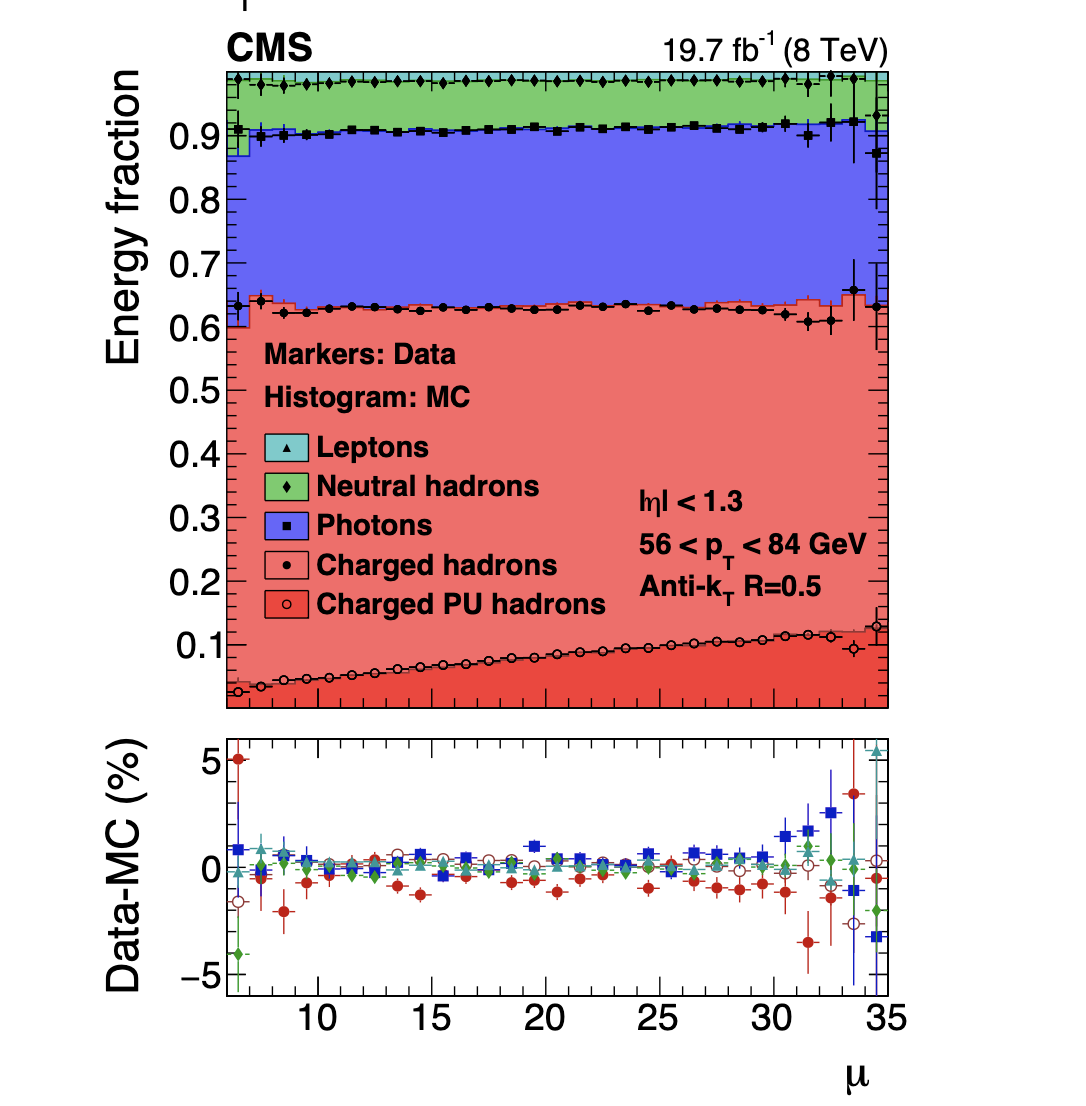
\includegraphics[width=0.75\textwidth]{figures/pfvalidation_mu_replace}
\caption{Comparison of number of pileup vertices in MC and Data~\cite{CMS-PRF-14-001}}
\label{fig:pfval_mu}
\end{figure}


\section{Top Tagging}
\label{sec:toptagging}

When a jet is boosted, the substructure can be exploited for tagging. Taggers apply criteria meant to separate signal jets from background. Machine Learning can also be applied to improve tagging abilities. In this analysis, the DeepAK8 mass decorrelated tagger is used~\cite{CMS:2020poo}. DeepAK8 is a machine learning tagger that takes a list of particle information and a list of secondary vertex information as inputs. The lists are then processed separately by 1 dimensional convolutional neural networks, then the outputs of the two separate layers are used as inputs in a fully connected layer, shown in Figure~\ref{fig:deepak8}.

Since many particle features are correlated with mass, the CNN is able to extract the mass of the jets. In some cases, a tagger needs to be independent of the mass of the jet. In this analysis, the background estimate uses the softdrop mass as an input, and so a tagger that does not bias the mass distribution is needed.

DeepAK8 has a mass decorrelated version which is developed by adding and additional mass prediction neural network. This mass prediction network calculates the accuracy of the CNN do extract the mass of the jet, and penalizes the tagger when the accuracy his high. 


\begin{figure}[h]
\centering
	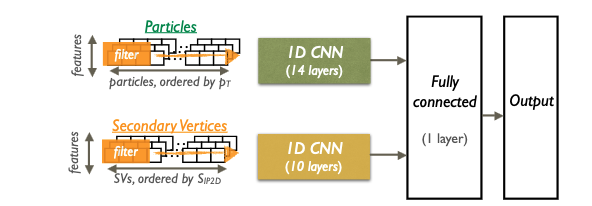
\includegraphics[width=0.8\textwidth]{figures/deepak8.png}
	\caption{Diagram of the DeepAK8 neural network.}
	\label{fig:deepak8}
\end{figure}


